% vim: set textwidth=78 autoindent:
% !TeX root = user_guide.tex

\section{Oracle GeoRaster Plugin}
\label{sec:oracleraster}
\index{Oracle-GeoRaster}

% when the revision of a chapter has been finalized, 
% comment out the following line:
% \updatedisclaimer

Oracle Datenbanken mit Oracle Spatial Erweiterung erm�glichen es, Rasterlayer
als SDO\_GEORASTER Objekte zu speichern. In QGIS existiert das
\toolbtntwo{oracle_raster}{Oracle GeoRaster Plugin}. Es basiert auf der GDAL
Bibliothek und setzt voraus, dass eine entsprechende Oracle Datenbank auf
ihrem Rechner l�uft. Obwohl Oracle keine freie Software ist, stellen Sie ihre
Software f�r Entwickler und zu Testzwecken kostenlos zur Verf�gung. Ein
einfaches Beispiel, wie man �ber GDAL ein Raster in eine Oracle Datenbank
laden kann sieht folgenderma�en aus:   
 
\filename{gdal\_translate -of georaster input\_file.tif geor:scott/tiger\@orcl}

Das Raster wird in diesem Beispiel in die Standard GDAL\_IMPORT Tabelle als
Spalte mit dem Namen RASTER geladen.

\subsection{Mit der Datenbank verbinden}

Als erstes muss das Oracle GeoRaster Plugin mit dem Plugin Manager geladen
werden (siehe Kapitel~\ref{sec:load_core_plugin}). Wenn Sie zum ersten Mal
ein GeoRaster in QGIS laden wollen, m�ssen Sie zuvor eine Verbindung zu der
Oracle Datenbank erstellen, in der sich die Daten befinden. Hierzu klicken
Sie auf das \toolbtntwo{oracle_raster}{Oracle Spatial GeoRaster w�hlen} Icon
in der Werkzeugleiste. In dem Dialog klicken Sie auf \button{Neu} und geben
dann die notwendigen Verbindungsparameter ein (siehe Abbildung
\ref{fig:oracle_create}) :  

\begin{itemize}[label=--]
\item \textbf{Name}: Geben Sie einen Namen f�r die Datenbankverbindung an.
\item \textbf{Datenbankinstanz}: Geben Sie den Namen der Datenbank an, mit
der Sie sich verbinden wollen.
\item \textbf{Benutzername}: Geben Sie den Benutzernamen an, mit dem Sie auf
die Datenbank zugreifen wollen.
\item \textbf{Passwort}: Das Passwort f�r den Benutzernamen, um auf die
Datenbank zuzugreifen.
\end{itemize}

\begin{figure}[ht]
   \begin{center}
   \caption{Dialog zum Erstellen einer Oracle Anbindung \nixcaption}\label{fig:oracle_create}\smallskip
   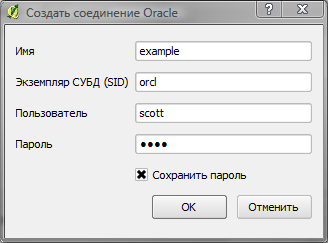
\includegraphics[clip=true, width=8cm]{oracle_create_dialog}
\end{center}
\end{figure}

Zur�ck im Hauptfenster des Oracle Spatial GeoRaster Plugins (siehe
Abbildung~\ref{fig:oracle_select}), w�hlen Sie die Dropdown Liste, um die
neue Verbindung auszuw�hlen und klicken dann auf \button{Verbinden}, um die
Verbindung herzustellen. Sie k�nnen die Verbindung auch nochmals
\button{Bearbeiten} und Ver�nderungen vornehmen oder mit dem Knopf
\button{L�schen} die Verbindung aus der Dropdown Liste entfernen.

\subsection{Ein GeoRaster ausw�hlen}

Wenn die Verbindung zur Datenbank steht, werden im Fenster 'Unterdaten' die
Namen aller Tabellen in Form eines GDAL 'subdataset' angezeigt, in
denen GeoRaster Spalten vorliegen.

W�hlen Sie einen der 'subdatasets' und klicken dann auf \button{W�hlen}, um
den Tabellennamen auszuw�hlen. Daraufhin erscheint eine weitere Liste mit den
GeoRaster Spalten, die sich in der Tabelle befinden. Dies ist normalerweise
eine kurze Liste, da es eher selten vorkommt, dass mehr als ein oder zwei
GeoRaster Spalten in einer Tabelle abgelegt sind. 

W�hlen Sie wieder einen der 'subdatasets' und klicken auf \button{W�hlen}, um
eine Tabellen/Spalten Kombination auszusuchen. Der Dialog zeigt die
Zeilen, die GeoRaster Objekte enthalten. Beachten Sie, dass in der Liste der
'subdatasets' nun die Rasterdatentabelle und Raster Id Paare angezeigt
werden. 

Es ist �brigens zu jeder Zeit m�glich, die Auswahl zu editieren, um so direkt
zu einem bereits bekannten GeoRaster oder zur�ck zum Anfang zu gelangen.    

\begin{figure}[ht]
   \begin{center}
   \caption{Dialog zum Ausw�hlen eines Oracle GeoRasters \nixcaption}\label{fig:oracle_select}\smallskip
   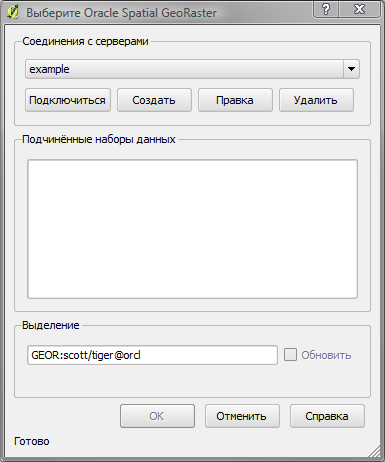
\includegraphics[clip=true, width=8.5cm]{oracle_select_dialog}
\end{center}
\end{figure}

Der Auswahlbereich kann auch dazu verwendet werden, um eine Where-Abfrage am
Ende der Identifikation hinzuzuf�gen, z.B.:
\filename{geor:scott/tiger@orcl,gdal\_import,raster,geoid=}. Weitere
Informationen finden Sie unter der URL
\url{http://www.gdal.org/frmt_georaster.html}.

\subsection{Ein GeoRaster laden}

Schlie�lich, wenn Sie aus der Liste der 'subdatasets' die Rasterdatentabelle
und Raster Id Paare ausgew�hlt haben, wird das entsprechende GeoRaster in
QGIS geladen.

Der Dialog zum Ausw�hlen eines Oracle GeoRasters kann nun geschlossen werden.
Beim n�chsten Aufruf wird die Verbindung wieder angezeigt mit derselben Liste
vorhandener 'subdatasets', so dass es einfach ist, weitere GeoRasters zu
laden.

\textbf{Bemerkung:} GeoRaster, die mit Pyramiden abgelegt sind, werden in
QGIS wesentlich schneller visualisiert. Die Pyramiden m�ssen aber im Vorfeld
und au�erhalb von QGIS mit Oracle PL/SQL oder gdaladdo erstellt werden.

Beispiel zum Erstellen von Pyramiden mit gdaladdo:

\begin{verbatim}
gdaladdo georaster:scott/tiger@orcl,georaster\_table,georaster,georid=6 -r 
nearest 2 4 6 8 16 32
\end{verbatim}

Beispiel zum Erstellen von Pyramiden mit PL/SQL: 

\begin{verbatim}
$ sqlplus scott/tiger
SQL> DECLARE
    gr sdo_georaster;
BEGIN
    SELECT image INTO gr FROM cities WHERE id = 1 FOR UPDATE;
    sdo_geor.generatePyramid(gr, 'rLevel=5, resampling=NN');
    UPDATE cities SET image = gr WHERE id = 1;
    COMMIT;
END;
/
\end{verbatim}

\FloatBarrier

